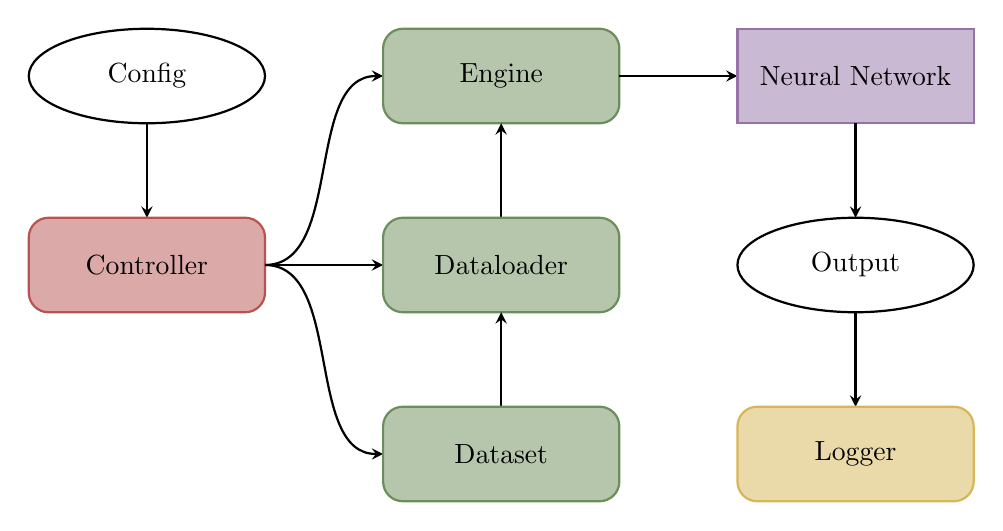
\begin{tikzpicture}[thick, yscale=.8]
	\definecolor{pink}{RGB}{184, 84, 80}
	\definecolor{blue}{RGB}{108, 142, 91}
	\definecolor{purple}{RGB}{150, 115, 166}
	\definecolor{yellow}{RGB}{214, 182, 86}
	
	% \drawroundedrectangle#x#y#width#height#corner#color$label
	\def\drawroundedrectangle#1#2#3#4#5#6#7{
		\fill[#6, fill opacity=.5, draw=#6, rounded corners=#5cm] (#1, #2) -- ++ (#3, 0) -- ++ (0, #4) -- ++(-#3, 0) -- cycle;
		\node at (#1 + #3 / 2, #2 + #4 / 2) {#7};
	}
	
	% \drawellipse#xcenter#ycenter#radiuswidth#radiusheight#label
	\def\drawellipse#1#2#3#4#5{
		\draw  (#1, #2) ellipse (#3 and #4) node {#5};
	}
	
	% diagram
	\drawellipse{1.5}{8.75}{1.5}{0.75}{Config}
	\draw[-stealth] (1.5, 8) -- (1.5, 6.5);
	\drawroundedrectangle{0}{5}{3}{1.5}{.25}{pink}{Controller}
	\draw[-stealth] (3, 5.75) .. controls (4, 5.75) and (3.5, 8.75) .. (4.5, 8.75);
	\draw[-stealth] (3, 5.75) -- (4.5, 5.75);
	\draw[-stealth] (3, 5.75) .. controls (4, 5.75) and (3.5, 2.75) .. (4.5, 2.75);
	\drawroundedrectangle{4.5}{8}{3}{1.5}{.25}{blue}{Engine}
	\draw[-stealth] (6, 6.5) -- (6, 8);
	\drawroundedrectangle{4.5}{5}{3}{1.5}{.25}{blue}{Dataloader}
	\draw[-stealth] (6, 3.5) -- (6, 5);
	\drawroundedrectangle{4.5}{2}{3}{1.5}{.25}{blue}{Dataset}
	\draw[-stealth] (7.5, 8.75) -- (9, 8.75);
	\drawroundedrectangle{9}{8}{3}{1.5}{0}{purple}{Neural Network}
	\draw[-stealth] (10.5, 8) -- (10.5, 6.5);
	\drawellipse{10.5}{5.75}{1.5}{0.75}{Output}
	\draw[-stealth] (10.5, 5) -- (10.5, 3.5);
	\drawroundedrectangle{9}{2}{3}{1.5}{0.25}{yellow}{Logger}
\end{tikzpicture}